\documentclass[10pt]{article}

% Minimal packages for fast compile
\usepackage{times}
\usepackage[utf8]{inputenc}
\usepackage[T1]{fontenc}
\usepackage[a4paper,margin=2cm]{geometry}
\usepackage{titlesec}
\usepackage{graphicx}
\usepackage{booktabs}
\usepackage{float}
\usepackage[section]{placeins}
\usepackage{setspace}

% Section title styles
\titleformat{\section}{\bfseries\fontsize{12}{14}\selectfont}{\thesection.}{0.5em}{}
\titleformat{\subsection}{\bfseries\fontsize{11}{13}\selectfont}{\thesubsection.}{0.5em}{}

% Custom title page
\begin{document}

\begin{titlepage}
\centering
\vspace*{2cm}

\includegraphics[width=0.3\textwidth]{image.png}
\vspace{1cm}

{\Huge\bfseries Status Report\par}
\vspace{2cm}

\begin{flushleft}
\textbf{Name of submission:} Status report 2\\[0.5em]
\textbf{Group name:} Testbench for Bit-Serial RISC-V processor in SoI for Venus\\[0.5em]
\textbf{Date:} 2025/12/02\\[0.5em]
\textbf{Organization:} KTH\\[1.5em]
\textbf{Authors:}\\[0.5em]
\begin{center}
\begin{tabular}{p{5cm}p{6cm}}
\toprule
\textbf{Name} & \textbf{Email} \\
\midrule
Chinmay Purandare & \texttt{chinmayp@kth.se} \\
Lorenzo Parata & \texttt{parata@ug.kth.se} \\
Chongnan Wang & \texttt{chongnan@kth.se} \\
Xiaotian Jiang & \texttt{xjia@kth.se} \\
Xinxin Qin & \texttt{xinxinq@kth.se} \\
Paul Martin & \texttt{paulmart@kth.se} \\
\bottomrule
\end{tabular}
\end{center}
\vspace{1em}
\end{flushleft}

\vfill
\begin{flushright}
\textbf{Department of Electronics}\\
KTH Royal Institute of Technology\\
Stockholm, Sweden
\end{flushright}
\end{titlepage}

% Table of Contents on separate page
\clearpage
\tableofcontents
\thispagestyle{plain}
\clearpage

% Start main content
\section{General description of status} 

During the recent sprints, the testbench subgroup focused heavily on the functional verification of the RISC-V processor core. To ensure comprehensive coverage, CoreMark was selected as the primary benchmark test case. A critical achievement during this phase was the identification and resolution of a logic bug within the Load-Store Unit (LSU), which was previously causing incorrect memory access behaviors.

Following the fix of the LSU, the RISC-V core has been successfully verified in the simulation environment. The processor is now able to execute the CoreMark benchmark correctly, confirming the logical correctness of the core architecture before moving to the final hardware integration phase.

In parallel, the bit-serial interface subgroup made substantial progress in defining the communication protocol between the two FPGA boards. The team established clear specifications for frequency requirements, pin assignments, and data transmission patterns. RTL implementation of the serial converter has been completed and undergoes continuous refinement based on simulation results. This module will serve as the critical bridge enabling the testbench to communicate with the processor under the severe I/O pad constraints imposed by the Venus mission requirements.

Cross-team coordination has improved significantly compared to earlier phases. Regular integration meetings ensure that both subgroups remain aligned on interface specifications and timing requirements. Documentation quality has also increased, with the README file restructured to better reflect the current codebase complexity and facilitate onboarding for future contributors.

The project timeline remains on track despite some anticipated delays in system-level integration. Buffer time allocated during initial planning has proven valuable in absorbing unforeseen technical challenges, particularly those related to clock domain crossing between the two FPGAs. The team has identified potential synchronization issues early and is actively working on handshake protocols and synchronizer circuits to mitigate timing inconsistencies.

Looking ahead to the final phase, the primary focus will shift toward full-system integration and on-board validation. Both major branches—testbench verification infrastructure and bit-serial communication—have reached functional readiness in their respective simulation environments. The upcoming sprints will concentrate on merging these components, conducting hardware-level testing, and collecting performance metrics to evaluate the feasibility of bit-serial processing for space applications.
\section{Resource Status}
\subsection{Time and Effort}
After resolving the initial issues in the codebase and becoming gradually familiar with the project structure, the team concentrated during the last four sprints on engineering development and technical documentation. This focus enabled steady progress in both the testbench development and the bit-serial interface branches as the project transitioned from preparation to active implementation.
In the testbench branch, three members worked on functional testing, coremark generation, and integrating the testbench with RAM and UART on the SoC. These tasks formed the core of the verification flow and significantly improved the maturity of the testbench.
In the bit-serial interface branch, the other three members concentrated on defining frequency and pin properties, specifying the communication protocol, and implementing the RTL. This work ensured that the communication mechanism can operate under the expected I/O limitations.

The cumulative time contribution per member and sprint is summarized below:

\begin{table}[h!]
\centering
\begin{tabular}{lcccc}
\hline
\textbf{Member} & \textbf{Sprint 3} & \textbf{Sprint 4} & \textbf{Sprint 5} & \textbf{Sprint 6} \\
\hline
Chongnan Wang & 15h & 10h & 11h & 11h\\
Xinxin Qin & 12h & 11h & 7h & 14h \\
Paul Martin & 16h & 8h & 8h & 9h \\
Xiaotian Jiang & 10h & 14h & 5h & 10h \\
Chinmay Purandare & &  &  & \\
Lorenzo Parata & 16h & 10h &  8h& 7h\\
\hline
\end{tabular}
\caption{Time contribution per member and sprint.}
\end{table}

Overall, the team has spent approximately xx hours so far (still being finalized), showing an increase compared with the previous status report as the project entered a more intensive development phase.

\subsection{Budget and Economic Status}
As this is an academic course project, no financial budget is involved. Team members’ work is unpaid, and the necessary hardware resources are provided by the supervisor, likely obtained through educational sponsorships.
During the project, a few minor expenses occurred, such as purchasing power adapters for the boards and cables to connect the two FPGA boards. These were handled individually by team members, or replaced through simple alternatives such as soldered connections. Such small expenses did not significantly impact project progress or planning.

\subsection{Personnel}
The project currently consists of six active members, each contributing according to the agile sprint plan described above.
The team is divided into two subgroups: Chongnan, Xinxin, and Xiaotian work on the testbench, while Chinmay, Paul, and Lorenzo focus on the bit-serial converter.
This division has proven effective in keeping responsibilities clear and preventing overlap between tasks. Collaboration between the two subgroups has remained consistent, ensuring that integration work can proceed smoothly in later stages.

\subsection{Materials and Equipment}
Each team member is currently using one \textbf{DE0-Nano-SoC Development Kit}, a robust FPGA platform based on the Altera System-on-Chip (SoC) architecture. The board combines a dual-core ARM Cortex-A9 processor with programmable logic, enabling flexible and high-performance embedded system design. The kit includes DDR3 memory, analog-to-digital capabilities, and Ethernet connectivity, offering a complete environment for hardware-software co-design.
As the project progressed, a few additional accessories such as FPGA communication cables were required to support multi-board testing. These items ensured that essential connections and debugging steps could be completed without delays.

\subsection{Deliverables}
After the sixth sprint, the deliverables include: a simulation-validated testbench integrated with UART and RAM on the FPGA board, capable of providing stimuli to the DUT, collecting logs, communicating with the PC, and comparing against a golden log; and a custom serial communication module that enables interaction between the testbench and the CPU under limited pad conditions. These deliverables form the basis of the final integration stage and demonstrate that both major branches of the project have reached functional readiness.

\subsection{Outlook}
In the next stage of work, we will wrap up the project, complete the integration between the two modules and conduct on-board testing, as well as test and collect the final data.The upcoming tasks will focus on validating full-system functionality and ensuring that the testbench and CPU interact reliably under hardware conditions.



\section{Problems / Action plan}
Chinmay
• State the problems the sponsor and steering committee need to be aware of, and
proposals for action

\newpage
\section{Risks / Action plan}
Since the last risk analysis, the team has continued to monitor risks. Indeed, several risks have evolved along the development. That is why it is importante de do an updated section where we are going to present you the current situation.

\subsection{Follow-up of Risk Analysis}
During the last few springs, risk management has proven to be useful. Indeed, some of the risks we previously identified did occur but were handled with success.
\begin{itemize}
    \item \textbf{Verification coverage} - Testbench may not provide full functional testing, so we decided to use CoreMark for that. It is a standard benchmark developed to measure the performance of a processor's core. It’s a perfect fit for us because it provides a simple and quick way to compare different CPUs, especially those found in embedded systems.
    \item \textbf{Coordination and availability} - As we expected, the different schedules of the team members create delays in communication. We manage this by writing reports on every meeting and by adapting the date of meetings accordingly to the team's availability.
    \item \textbf{Integration timeline underestimation} - fSystem-level testing has taken longer than expected. However, we are still on time thanks to the allocated buffer time we have set at the start of the project.
    \item \textbf{Extreme Environment} - After discussion with our professor, making our FPGA resistant to extreme environments is not a requirement for our project. Indeed, another team will probably in the future work on this aspect by selecting different materials and applying triplication techniques to protect the design from radiation.
\end{itemize}

\subsection{Updated Risk Analysis}
Here is the new version of our risk analysis table and matrix. To simplify, we erased the ones that became insignificant during our previous analysis, that is to say risks 4, 12, 8, 13, 9. We have also updated a few risks and added new ones.
\begin{table}[h!]
\centering
\begin{tabular}{|c|p{2.35cm}|p{4.1cm}|c|c|c|p{4.3cm}|p{1.17cm}|c|}
\hline
\textbf{ID} & \textbf{Risk} & \textbf{Description} & \textbf{P} & \textbf{C} & \textbf{R} & \textbf{Suggested Action} & \textbf{Follow-up Date} & \textbf{Trend} \\
\hline
1 & Hardware complexity & Two processor models on separate FPGAs increase design and debugging effort. & 3 & 4 & 12 & Start with single-FPGA setup, define early comm. protocols. & 31 Oct & $\downarrow$ \\
\hline
2 & Multi-FPGA system complexity & Communication and timing between boards difficult to synchronize. & 4 & 4 & 16 & Test modules separately, simulate before hardware link. & 31 Oct & $\rightarrow$ \\
\hline
3 & Extreme environment & SoI may not survive Venus-like temperatures. & 2 & 5 & 10 & Study environmental limits; keep simulation-level validation. & 28 Nov & $\downarrow$ \\
\hline
5 & Performance gap & Bit-serial version may not reach required speed. & 4 & 3 & 12 & Define realistic targets, compare to parallel baseline. & 31 Oct & $\rightarrow$ \\
\hline
6 & Verification coverage & Testbench may not provide full functional testing. & 3 & 5 & 15 & Add random/stress test patterns; document coverage. & 28 Nov & $\downarrow$ \\
\hline
7 & Specialized toolchain dependency & ProGram compiler unstable or limited. & 3 & 3 & 9 & Validate early, keep VHDL rewrite backup plan. & 24 Oct & $\downarrow$ \\
\hline
10 & Internal conflicts & Potential disagreements between members. & 3 & 4 & 12 & Address through discussion or reassigning tasks. & 31 Oct & $\rightarrow$ \\
\hline
11 & Integration timeline underestimation & System-level testing may take longer than expected. & 5 & 3 & 15 & Allocate buffer time, set MVP milestone. & 31 Oct & $\rightarrow$ \\
\hline
14 & Clock domain and timing inconsistencies & Different clocks between the two FPGAs can cause missed pulses or unreliable data transfers. & 4 & 4 & 16 & Define a clear clocking strategy. Add synchronizers, handshake protocols or even PLL if needed. & 28 Nov & $\uparrow$ \\
\hline
\end{tabular}
\caption{Mini Risk Method Table}
\end{table}

\begin{figure}[h!]
    \centering
    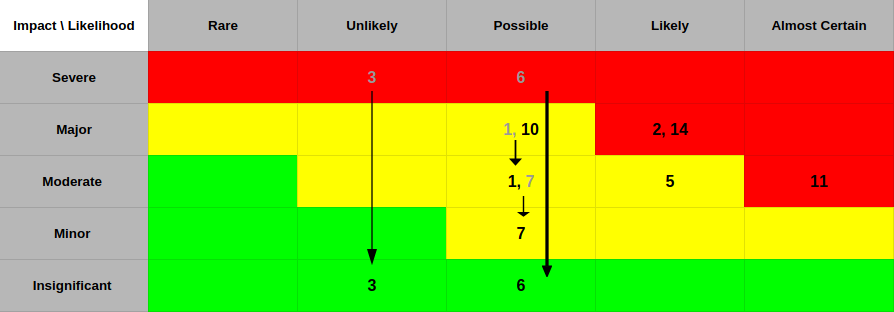
\includegraphics[width=1\textwidth]{risk_matrix_v2.png}
    \caption{Updated Risk Matrix}
\end{figure}

\subsection{Risks to Be Reported}

According to the current risk matrix, 3 risks are currently considered highly critical for the project (in the red zone) and need important attention. 

We have especially Risk 2 – Multi-FPGA System Complexity and Risk 11 – Integration Timeline Underestimation that remain an important concern, as we already talk about in the previous status report.

But we have in addition Risk 14 – Clock Domain and Timing Inconsistencies that is new. During multi-FPGA integration, even small clock differences between the processor board and the testbench board can lead to errors. However, the 2 FPGAs do not share the exact same clock and it might lead to timing drift and signal synchronization issues. To avoid this, it is important to have proper synchronizers and handshake logic. In the worst case scenario, we might even need to implement an PLL.


\section{Project changes from the project plan}

The following table documents the deviations from the original project plan. It highlights new technical requirements, hardware prerequisites, documentation updates, and organizational adjustments to ensure project transparency.

\begin{table}[h!]
    \centering
    \renewcommand{\arraystretch}{1.6} %稍微增加行高以容纳更多内容
    \begin{tabular}{|p{0.18\textwidth}|p{0.42\textwidth}|p{0.32\textwidth}|}
        \hline
        \textbf{Change Type} & \textbf{Description} & \textbf{Impact / Action Plan} \\
        \hline
        
        \textbf{New Requirement} & 
        \textbf{Cross-Platform Compatibility} \newline 
        Code discrepancies between Windows and Linux (e.g., makefile paths, library dependencies) caused build failures. & 
        Refactored build scripts and standardized compiler flags to ensure seamless portability across both OS environments. \\
        \hline
        
        \textbf{Changed Requirement} & 
        \textbf{Testbench Scope Expansion} \newline 
        Validation now requires functional coverage for both RISC-V and CISC-V architectures to ensure instruction set compatibility. & 
        Refactoring verification logic to support dual-architecture testing and implementing automated regression tests. \\
        \hline
        
        \textbf{New Prerequisite} & 
        \textbf{Hardware Interconnection} \newline 
        Identified a missing specific female-to-female interface required to bridge the two development boards for signal transmission. & 
        Team will fabricate (solder) a custom cable to meet connection requirements immediately to avoid blocking hardware integration. \\
        \hline
        
        \textbf{Changed Organization} & 
        \textbf{Holiday Schedule Optimization} \newline 
        Reduced workforce availability during the upcoming Christmas break requires a shift in project phasing. & 
        Critical path tasks accelerated to be completed pre-holiday; remote workflow established for asynchronous contributions. \\
        \hline
        
        \textbf{New Document} & 
        \textbf{Documentation Overhaul (README)} \newline 
        The initial project documentation was insufficient for the current code complexity. & 
        Restructured `README.md` and added inline comments to improve code structure visibility and long-term maintainability. \\
        \hline
        
        \textbf{Clarified Requirement} & 
        \textbf{Specification Alignment} \newline 
        Initial hardware specifications contained ambiguities regarding interface details. & 
        Conducted a detailed review with the supervisor to define missing constraints; updated the hardware design specifications accordingly. \\
        \hline
        
    \end{tabular}
    \caption{Summary of Changes and Deviations from the Project Plan}
    \label{tab:project_changes}
\end{table}


\section{Appendix}
• Updated time plan\\
• Updated resource plan


\end{document}
